
\documentclass[13pt,compress]{beamer}
% deactivate beamer navigation
%\setbeamertemplate{navigation symbols}{}
%\usepackage{geometry}
%\geometry{papersize={180mm, 135mm}, top=-1.5mm} % 210mm, 297mm

\usepackage[nospeakermargin]{../style/lmu-lecture}

\setbeamertemplate{frametitle}{\expandafter\uppercase\expandafter\insertframetitle}
%\useoutertheme{metropolis}
% remove section slides
\AtBeginSection[]
{
  \begin{frame}<beamer>
    \frametitle{Part 1}
    \tableofcontents[currentsection]
  \end{frame}
}
% includepdf slides, pagecommad will set counter for framenumber
\usepackage{pdfpages}
\includepdfset{trim=0mm 0mm 0mm 0mm, pagecommand={\global\setcounter{framenumber}{\value{page}}}}
% trim=0mm 6mm 0mm 0mm, offset=0 15,
% add footer:
\usepackage{framed, color}
\usepackage{xcolor}
%\iffalse
% \setbeamertemplate{footline}[text line]{%
%     \noindent\hspace*{\dimexpr-\oddsidemargin-1in\relax}%
%      \colorbox{white}{
%      \makebox[\dimexpr\paperwidth-2\fboxsep\relax]{
%      \color{black}
%      \begin{minipage}[c][4.5ex][c]{0.5\linewidth}
%        \secname
%      \end{minipage}
%      \hfill\begin{minipage}[c][4.5ex][c]{0.5\linewidth}
%        \flushright
%        \insertframenumber{}~/~\inserttotalframenumber~~
%      \end{minipage}
%      }}%
%   \hspace*{-\paperwidth}
% }



% \setbeamertemplate{footline}[text line]{%
%     \noindent\hspace*{\dimexpr-\oddsidemargin-1in\relax}%
%      \colorbox{white}{
%      \makebox[\dimexpr\paperwidth-9ex\relax]{
%      \color{black}
%      \begin{minipage}[c][2.5ex][b]{0.5\linewidth}
%        \secname
%      \end{minipage}
%      \hfill\begin{minipage}[c][2.5ex][b]{0.5\linewidth}
%        \flushright
%        %\insertframenumber{}~/~\inserttotalframenumber~~
%      \end{minipage}
%      }}%
%      \begin{minipage}[c][3.5ex][t]{6.5ex}
%        \flushright
%        \fontsize{4pt}{6}\selectfont\transparent{0.3}\insertframenumber{}~/~\inserttotalframenumber~~
%      \end{minipage}
%   \hspace*{-\paperwidth}
% }
%\fi

\title{Introduction to Machine Learning\\with R and mlr3}
\author{Bernd Bischl \& Marvin N. Wright}
%\institute{Essential Data Science Training}
\date{DAGStat, March 2025}



\begin{document}
\setbeamercolor{background canvas}{bg=}

% General remark: hyperlinks in included pdfs are not clickable anymore in the combined pdf

\frame{\titlepage}

\includepdf[pages={4-7}, trim=0mm 0mm 45mm 0mm]{../slds-lecture-pdfs/lecture_i2ml/slides-pdf/slides-basics-whatisml.pdf}

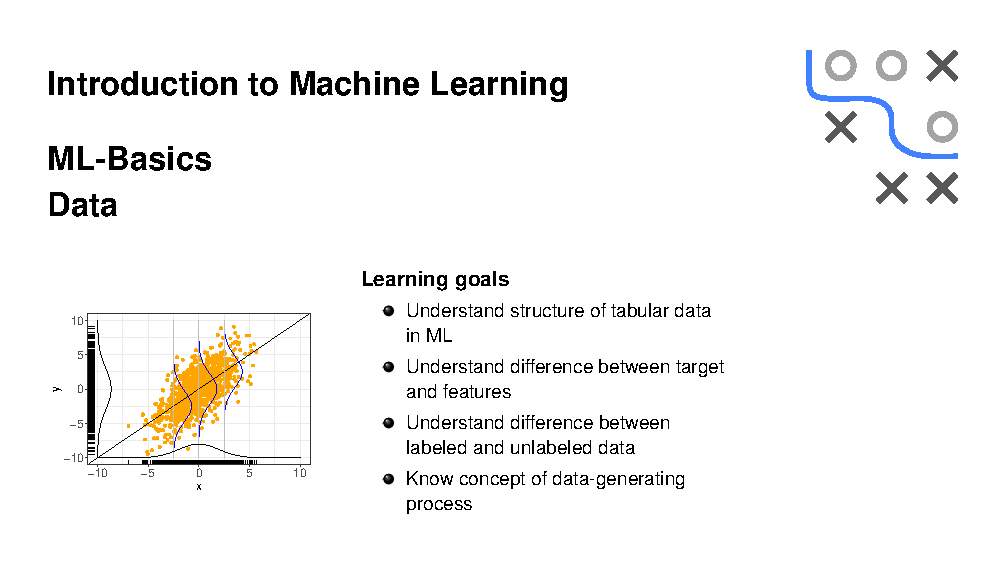
\includepdf[pages={1-9}, trim=0mm 0mm 45mm 0mm]{../slds-lecture-pdfs/lecture_i2ml/slides-pdf/slides-basics-data.pdf}

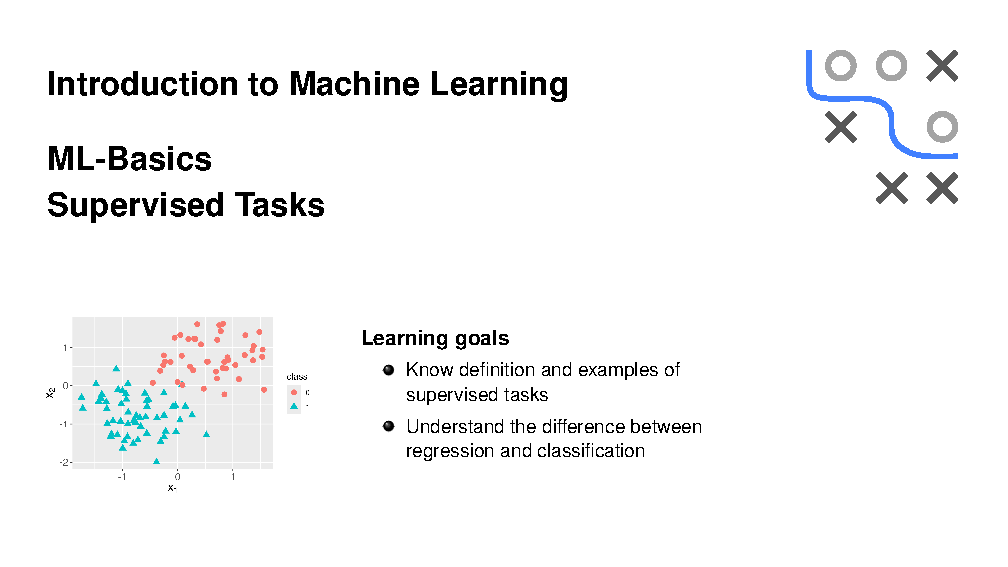
\includepdf[pages={1-last}, trim=0mm 0mm 45mm 0mm]{../slds-lecture-pdfs/lecture_i2ml/slides-pdf/slides-basics-task.pdf}

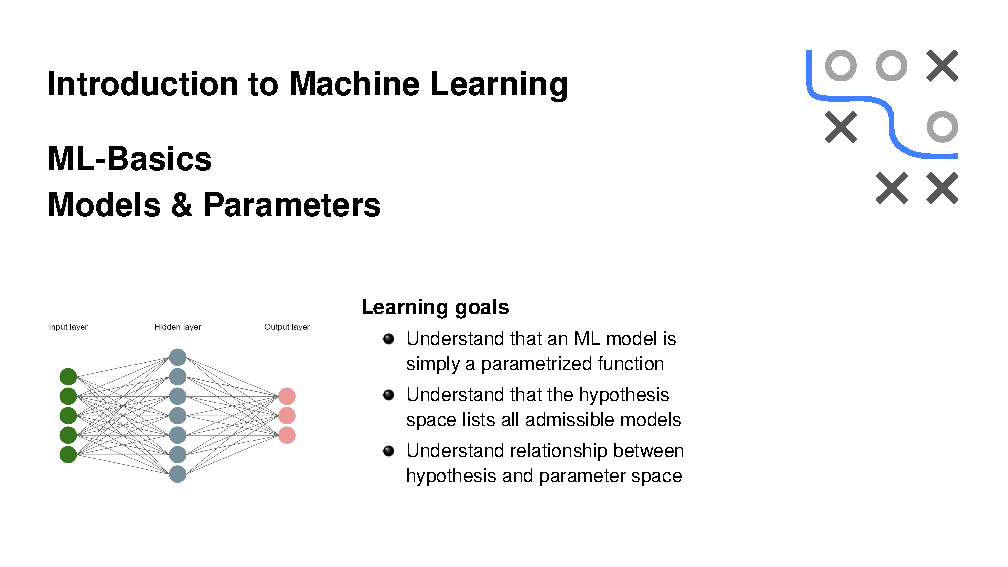
\includepdf[pages={1-9}, trim=0mm 0mm 45mm 0mm]{../slds-lecture-pdfs/lecture_i2ml/slides-pdf/slides-basics-models-parameters.pdf}

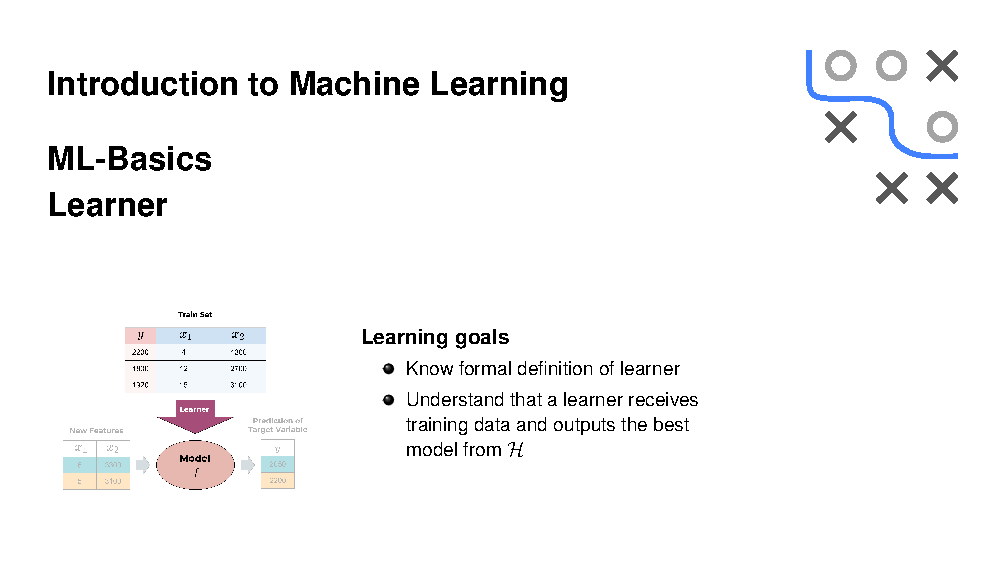
\includepdf[pages={1-last}, trim=0mm 0mm 45mm 0mm]{../slds-lecture-pdfs/lecture_i2ml/slides-pdf/slides-basics-learner.pdf}

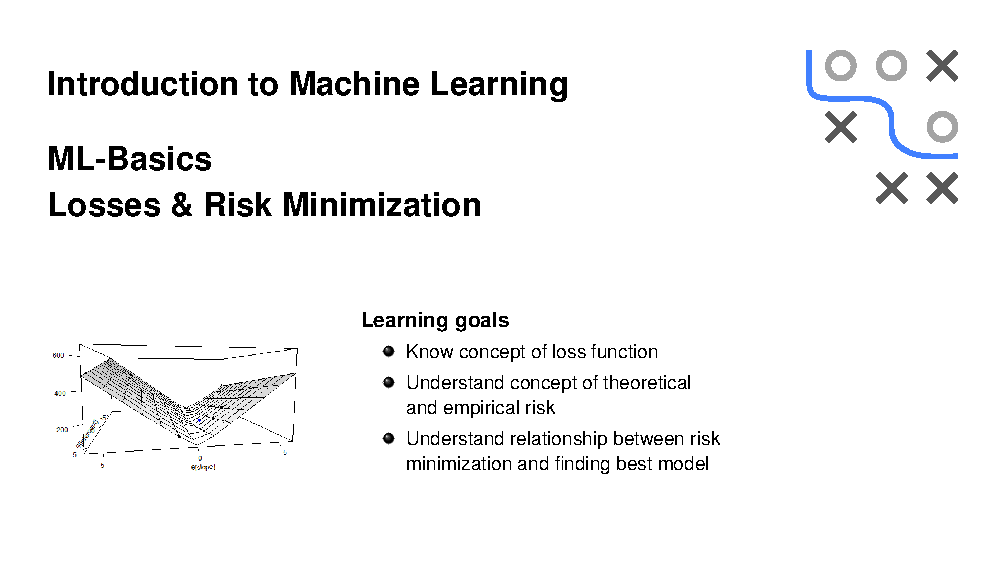
\includepdf[pages={1-last}, trim=0mm 0mm 45mm 0mm]{../slds-lecture-pdfs/lecture_i2ml/slides-pdf/slides-basics-riskminimization.pdf}

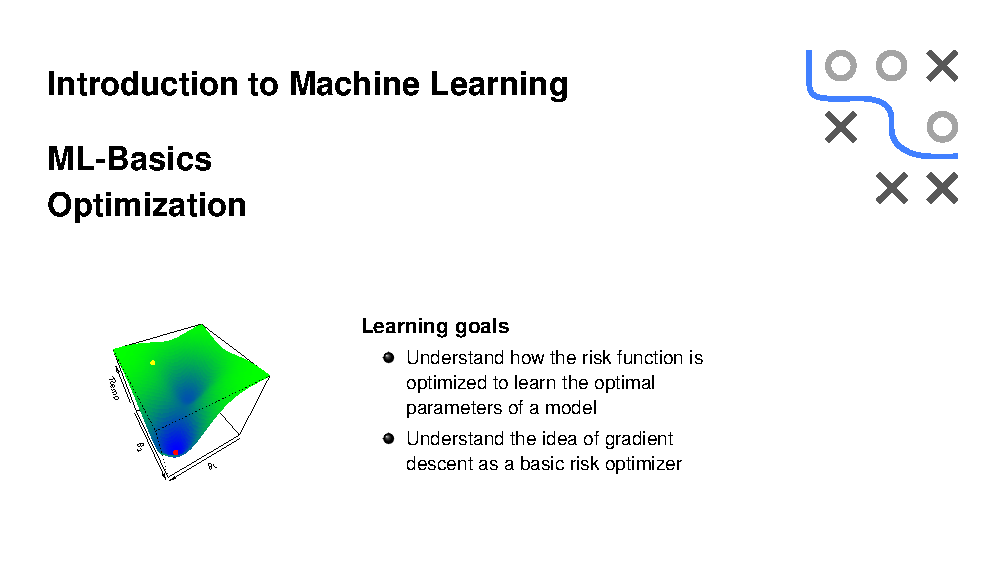
\includepdf[pages={1,2,6-9,11}, trim=0mm 0mm 45mm 0mm]{../slds-lecture-pdfs/lecture_i2ml/slides-pdf/slides-basics-optimization.pdf}

\includepdf[pages={1-5}, trim=0mm 0mm 45mm 0mm]{../slds-lecture-pdfs/lecture_i2ml/slides-pdf/slides-classification-tasks.pdf}

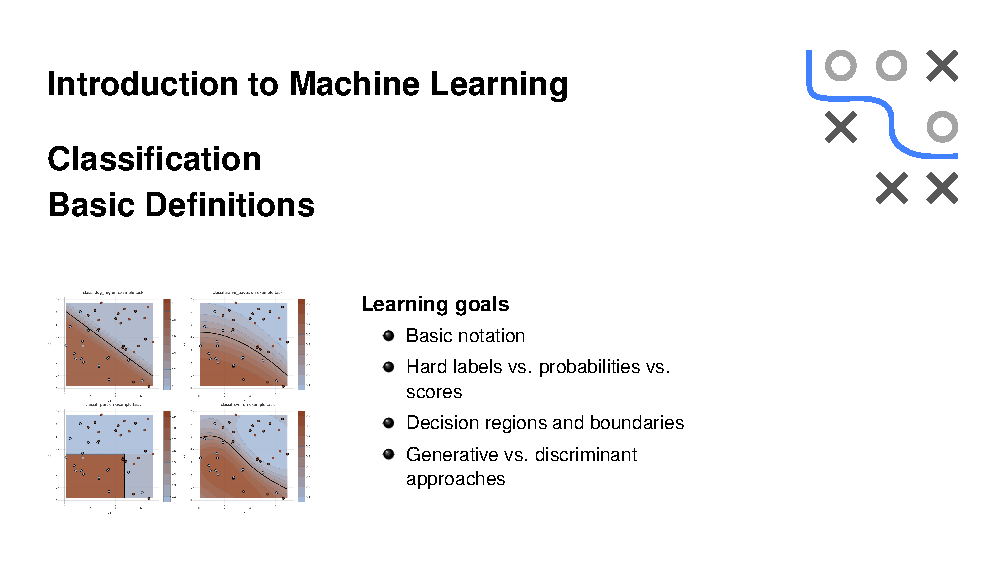
\includepdf[pages={1-9}, trim=0mm 0mm 45mm 0mm]{../slds-lecture-pdfs/lecture_i2ml/slides-pdf/slides-classification-basicdefs.pdf}

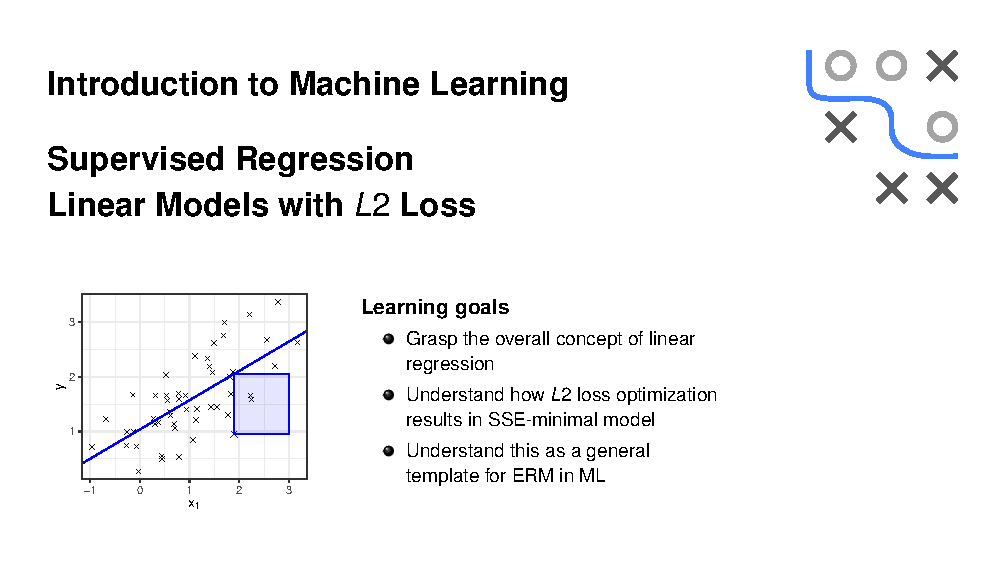
\includepdf[pages={1-5, 13}, trim=0mm 0mm 45mm 0mm]{../slds-lecture-pdfs/lecture_i2ml/slides-pdf/slides-regression-linearmodel-l2.pdf}

%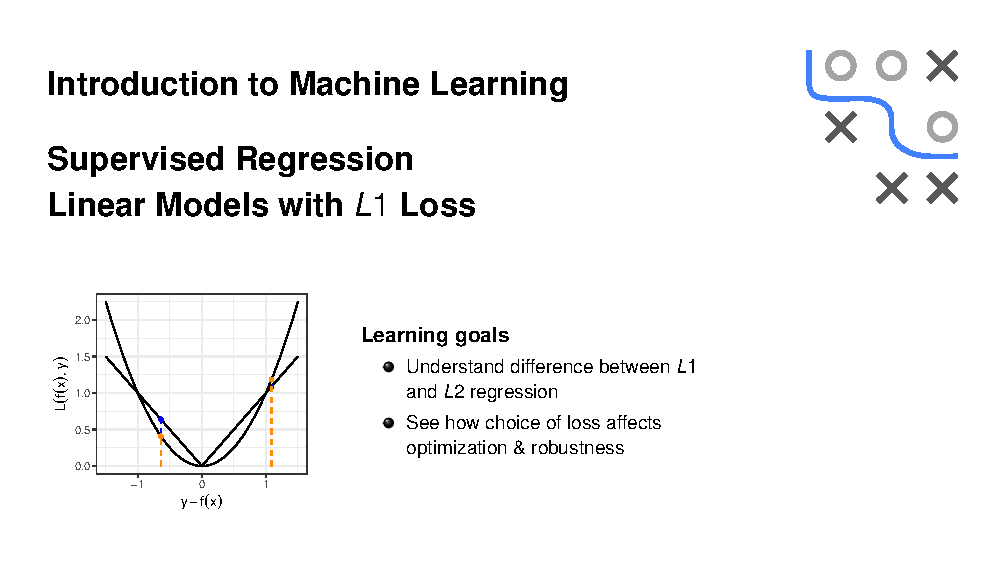
\includepdf[pages={1-last}, trim=0mm 0mm 45mm 0mm]{../slds-lecture-pdfs/lecture_i2ml/slides-pdf/slides-regression-linearmodel-l1.pdf}

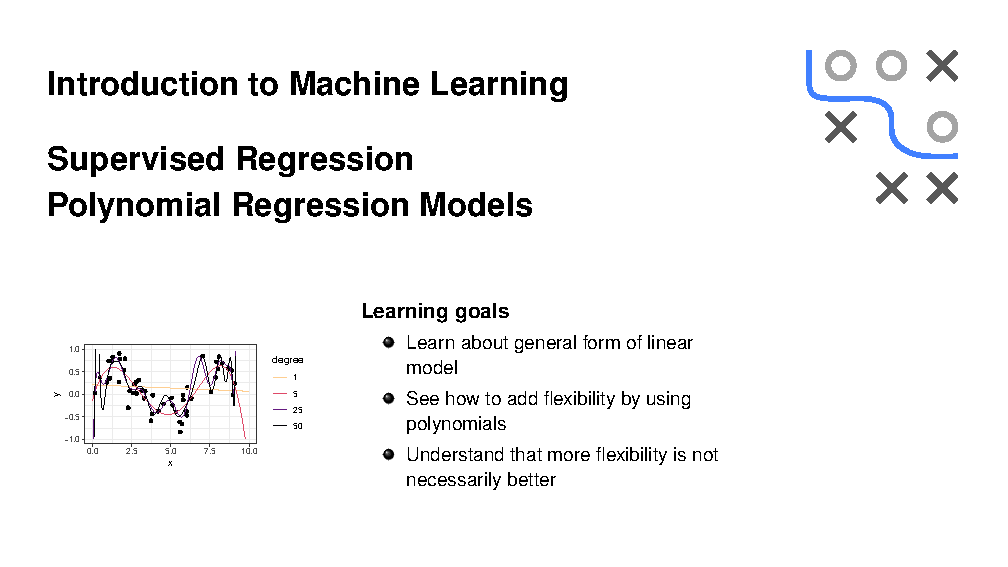
\includepdf[pages={1-6, 8-last}, trim=0mm 0mm 45mm 0mm]{../slds-lecture-pdfs/lecture_i2ml/slides-pdf/slides-regression-polynomials.pdf}

% 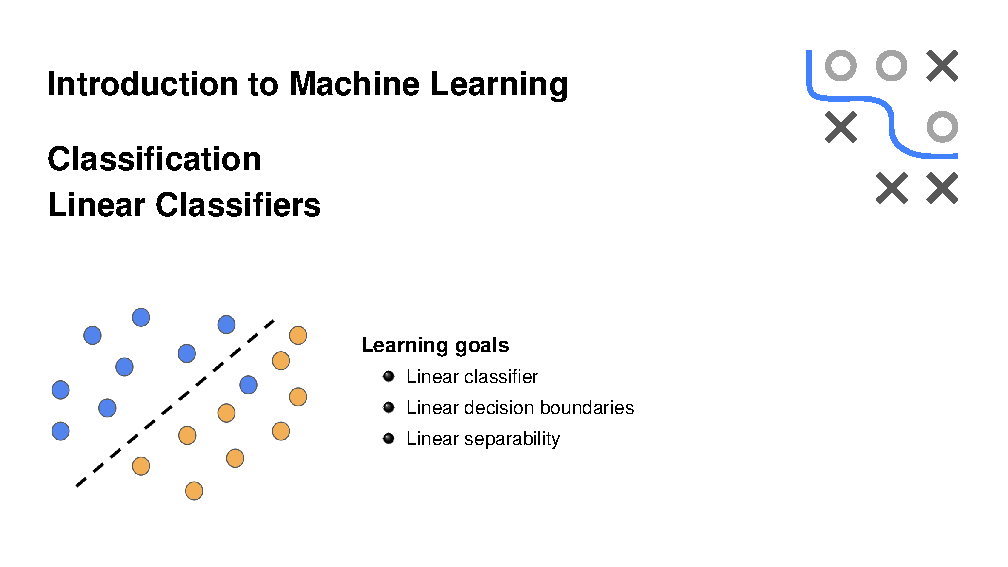
\includepdf[pages={1-last}, trim=0mm 0mm 45mm 0mm]{../slds-lecture-pdfs/lecture_i2ml/slides-pdf/slides-classification-linear.pdf}

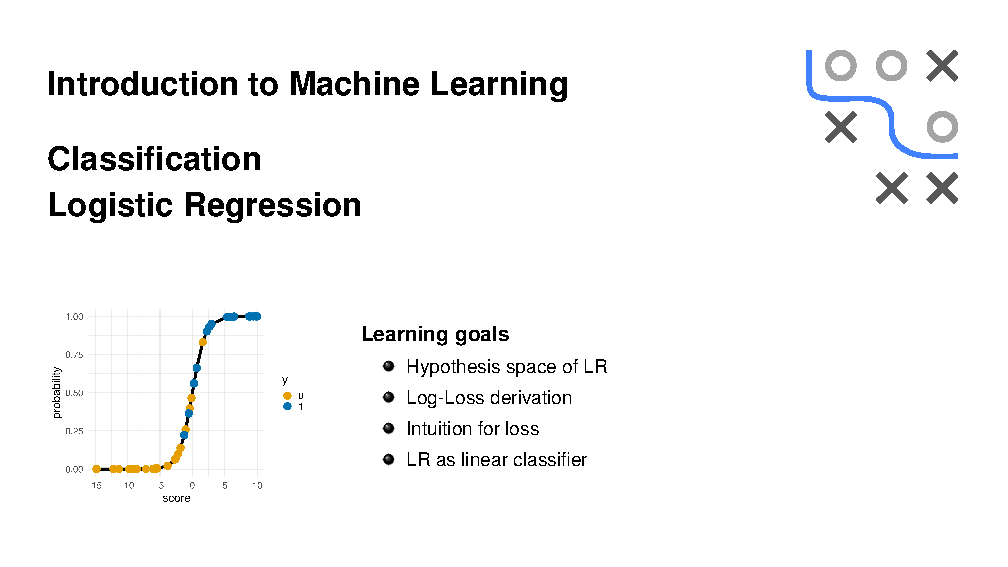
\includepdf[pages={1-4, 6-last}, trim=0mm 0mm 45mm 0mm]{../slds-lecture-pdfs/lecture_i2ml/slides-pdf/slides-classification-logistic.pdf}

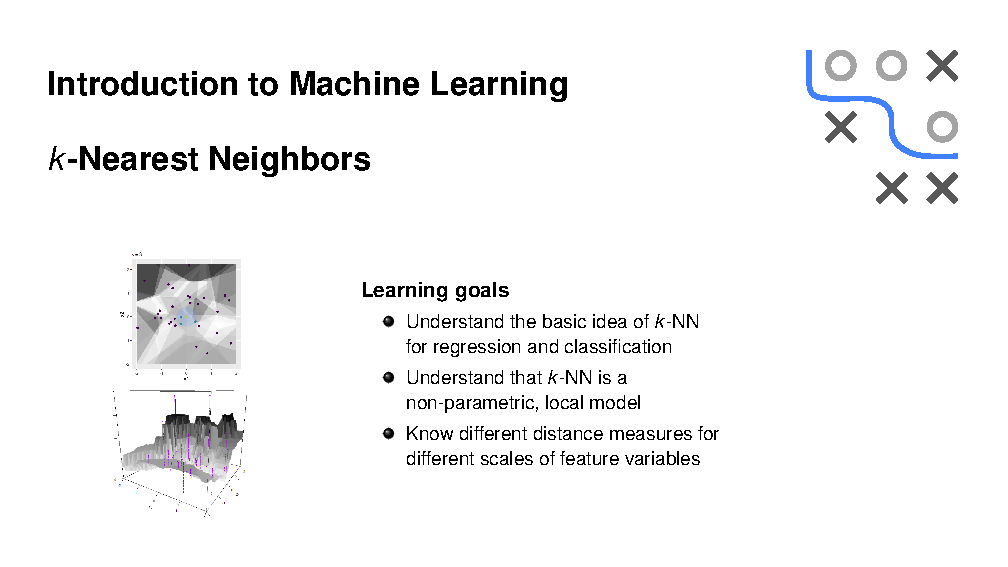
\includepdf[pages={1-8}, trim=0mm 0mm 45mm 0mm]{../slds-lecture-pdfs/lecture_i2ml/slides-pdf/slides-knn.pdf}



\end{document}
